% The original template (from Trevor) had a custom \appendix command,
% but I found it to break figure/table counters. I'm not sure how
% reliable my fix is, so I ended up reverting back to the standard
% latex version, and renaming the custom command to \myappendix.  You
% can try both and see how things work out:
% 1) Call \appendix once, and then make each appendix a \chapter
% 2) Call \myappendix once, and then make each appendix a \section.

\appendix

%%%%%%%%%%%%%%%%%%%%%%%%%%%%%%%%%%%%%%%%%%%%%%%%%%%%%%%%%%%%%%%%%%%%%%%

\chapter{Théorie de la promesse}
\label{appendix:promise_theory}

\section{Définition de la promesse}

Une promesse est différente d'un engagement : un engagement est le moment où un
agent rompt avec une ligne de conduite pour une autre discontinue avec des vues
sur un objectif, la plupart du temps à travers une action spécifique ou un
investissement sur des résultats futurs. Dans certains cas, l'acte
d'engagement peut résulter en une promesse persistante, mais promettre
n'implique pas une action provoquant un changement discontinu.

%{%\begin{figure}[H]
%    \centering
%    \begin{tabular}{l}
        ``Une promesse est la spécification d'un état ou comportement \\
        ultérieur d'un agent autonome à un autre. Elle est ainsi, \\
        une unité de politique.`` \cite{burgess_modeling_2006} \\
        %\em \footnotesize Mark Burgess, Alva Couch, Modeling Next Generation
        %Configuration Management Tools, \\
        %\em \footnotesize Pp. 131-147 of the Proceedings of LISA '06,
        %Décembre 2006
%    \end{tabular}
    %\caption{La promesse par Burgess et al. (2006)}
    %\label{fig:quote}
%\par}%\end{figure}

Les promesses sont faites à un agent par un agent et sont modélisées par une
relation unidirectionnelle labellisée par un \emph{corps} de promesse qui
définit la substance de la promesse. Une promesse avec le \emph{corps}
\textbf{+b} est une déclaration pour ''donner'' un comportement d'un agent à un
autre, tandis qu'une promesse avec le \emph{corps} \textbf{-b} est la
spécification de quel comportement sera reçu, accepté ou utilisé.

\section{Caractéristiques de la promesse}

Un promesse est l'annonce d'un fait ou d'un comportement d'un prometteur à un
promis, sous le regard d'un certain nombre de témoins (définissant le champ
d'application de la promesse), dont le résultat n'a pas encore été évalué.  On
distingue deux types de promesses :

\begin{itemize}
    \item Une promesse d'accepter de se comporter comme une autre. C'est
        essentiel pour la définition de groupes, de rôles ou de structures
        sociales avec un consensus de comportement (cf. section
        \ref{sec:consensus})
    \item Une promesse d'utiliser la promesse d'un autre. C'est crucial pour les
        interactions client/serveur, les dépendances et les contrôles d'accès.
\end{itemize}

Un promesse présente les caractéristiques suivantes :

\begin{enumerate}
    \item Il doit y avoir des agents pour qu'une promesse existe.
    \item Il doit y avoir un prometteur (ou agent source).
    \item Il doit y avoir un promis (ou agent destinataire), qui peut très bien
        aussi être la source.
    \item Il doit y avoir un \emph{corps} qui décrit la nature de la promesse.
\end{enumerate}

\section{Représentation et types de promesse: $\pi$-calculus}

\begin{table}[H]
    \begin{tabularx}{\textwidth}{
            >{\centering\arraybackslash}X|
            >{\centering\arraybackslash}X|
            >{\centering\arraybackslash}X|
        }

        \cline{2-3}
        & 
        \textbf{Notation} &
        \textbf{Interprétation} \\ 

        \cline{2-3}
        &
        $a \xrightarrow{+b} a'$ &
        Promesse avec le \emph{corps} $b$ \\

        &
        $a' \xrightarrow{-b} a$ &
        Promesse d'accepter $b$ \\

        &
        $v_a(a \xrightarrow{b} a')$ &
        La valeur de la promesse à $a$ \\

        \cline{1-1}
        \multicolumn{1}{ |X| }{\textbf{Type de promesse}} &
        $v_{a'}(a \xrightarrow{b} a')$ &
        La valeur de la promesse à $a'$ \\

        \cline{1-3}
        \multicolumn{1}{ |c| }{Basique} &
        $n_1 \xrightarrow{\pi} n_2$ &
        Fournit un service / un flux \\

        \multicolumn{1}{ |c| }{Coopérative} &
        $n_1 \xrightarrow{C(\pi)} n_2$ &
        Imite / Suit \\

        \multicolumn{1}{ |c| }{Utilisatrice} &
        $n_1 \xrightarrow{U(\pi)} n_2$ &
        Utilise / Accepte de la part de\\

        \multicolumn{1}{ |c| }{Conditionnelle} &
        $n_1 \xrightarrow{\pi_1/\pi_2} n_2$ &
        ``File`` de promesses: $\pi_1$ if $\pi_2$\\
        \cline{1-3}
    \end{tabularx}
    \caption{Représentation et types de promesses}
    \label{PromiseTypes}
\end{table}
   
Les promesses de service basiques forment un certain nombre de types, comme par
exemple `fournir un web service en moins de 5 millisecondes` ou `donner
n'importe quel information sur l'agent X`. D'autres exemples :

\begin{itemize}
    \item $X \xrightarrow{q \leq q_0} Y $: l'agent $X$ promet de ne jamais éxeder la
        limite $q \leq q_0$.
    \item $X \xrightarrow{q = q_0} Y $: l'agent $X$ promet de satisfaire
        $q = q_0$.
    \item $X \xrightarrow{\ell \subseteq  L} Y $: $X$ promet de garder $\ell$
        comme sous-langage du langage L
    \item $X \xrightarrow{S} Y $: $X$ offre le service $S$ à $Y$.
    \item $X \xrightarrow{R} Y $: $X$ promet de relayer $R$ à $Y$.
    \item $X \xrightarrow{\neg R} Y $: $X$ promet de ne jamais relayer $R$ à $Y$.
    \item $X \xrightarrow{S,t} Y $: $X$ promet de répondre avec le service $S$
        en l'espace de $t$ secondes.
\end{itemize}

Une promesse est dite ``rompue`` si un agent fait deux promesses contradictoires du
même type et en même temps (différent d'une promesse qui aurait expiré ou changé).

\section{Processus de raisonnement lié à la promesse}

Le procédé de raisonnement qui accompagne l'émanation d'un promesse, se divisent
en plusieurs sous-étapes, accrochez-vous:

\begin{itemize}
  \item \textbf{Préparation de la promesse} -
	Processus de raisonnement effectué par A conduisant à la conception, la
	synchronisation et la délivrance de la promesse P par A.
  \item \textbf{Analyse de crédibilité} -
	Processus de raisonnement où les agents C dans le champ d'application de
	la promesse P déterminent la crédibilité qu'ils assignent à A promettant
	P compte tenu des faits connus de A (mais à l'exception des informations
	historiques précises sur le comportement individuel d'un membre de sa
	classe d'agent)
  \item \textbf{Détermination préliminaire de la confiance} -
	Processus de raisonnement effectué par C (C dans le domaine
	d'application de la promesse P) servant à :
  	\begin{enumerate}
	  \item déterminer la confiance que C accorde à A avant même de
		  connaitre la promesse P (confiance préalable)
	  \item spécifier quelles sont les attentes générées par la prise en
		  considération de la promesse P.
  	\end{enumerate}
  \item \textbf{Délibération de contre-promesse} -
	Processus de raisonnement effectué par B concernant les contre-promesses
	pouvant potentiellement être émises par B en retour de considération de
	P (B dans le champ d'application de P)
  \item \textbf{Prédiction de l'impact de la promesse} -
	(cela peut être réalisé à condition que B ait émis une ou plusieurs
	contre-promesses plausibles)
  	\begin{enumerate}
	  \item Processus de raisonnement effectué par B (dans le champ
		  d'application de P) et C (n'importe quel agent dans le champ
		  d'application de P) servant à déterminer les (le changement
		  des) attentes que P créé dans B (et que A a l'intention de
		  générer).  
	  \item Processus de raisonnement visant à la modification des ententes
		  (détenues par B ou C) étant donné la changement des attentes
		  de chacun d'entre eux amené par la prise en considération de
		  la promesse P.
  	\end{enumerate}
  \item \textbf{Évaluation de la promesse} -
	Processus de raisonnement effectué par C concernant :
  	\begin{enumerate}
	  \item la façon dont C va évaluer si la promesse de A a été tenue ou
		  non.
      \item l'évaluation de cette dernière au moyen de la méthode la plus
          adéquate
  	\end{enumerate}
  \item \textbf{Surveillance de rétraction de promesse} -
	A peut être amené à un stade ultérieur à émettre une autre promesse Q,
	pour laquelle la tenue n'est pas compatible avec la tenue de P. Dans ce
	cas, Q qualifie un retrait de P. Un agent C applique un processus de
	raisonnement qui surveille et évalue les promesses postérieures émises
	par A pour déterminer si celles-ci seront amenées à rompre la promesse P
	et induire sont retrait.
  \item \textbf{Mise à jour de la confiance} -
	Processus de raisonnement en place pour chacun des agents C dans le champ
	d'application de P visant à mettre à jour la confiance préalablement
	accordée à A, en adéquation avec la résultat de l'évaluation que C fait
	concernant le degré avec lequel la promesse P a été tenue par A.
  \item \textbf{Critère de réputation} -
	Processus de raisonnement effectué par chacun des agents C dans le champ
	d'application de P visant à échanger entre les différent agents les
	effets des mises à jour de confiance. Le flux de réputation permet a un
	agent C n'ayant aucuns aprioris sur un agent A d'acquérir une confiance
	initiale en prenant en considération les preuves recueillies par les
    autres agents (parce que même les agents ont des casiers judiciaires).
\end{itemize}

%%%%%%%%%%%%%%%%%%%%%%%%%%%%%%%%%%%%%%%%%%%%%%%%%%%%%%%%%%%%%%%%%%%%%%%

\chapter{Consensus de Raft}
\label{appendix:consensus}

\section{États des serveurs}

Un cluster Raft comprend une multitude des serveurs (cinq est un nombre courant
permettant au système de tolérer deux échecs). À n'importe quel moment donné,
chacun des serveur est dans l'un de ces états :

\begin{itemize}
    \item \textbf{Leader} -
        En cycle normal, il existe un et un seul \emph{leader} et tous les autres
        serveurs sont \emph{followers}. Le \emph{leader} traite les requêtes de
        tous les clients (si un client contacte un \emph{follower}, le
        \emph{follower} le redirige vers le \emph{leader}).
    \item \textbf{Follower} -
        Les \emph{followers} sont passifs : ils n'émettent jamais de messages par
        leur propre initiative, ils se contentent simplement de répondre aux
        requêtes émises par le \emph{leader} et les \emph{candidats}.
    \item \textbf{Candidat} -
        Statut intermédiaire utilisé lors de l'élection d'un nouveau
        \emph{leader}. La figure \ref{fig:raft_server_states} montre les différents états
        et transitions possibles dans un cluster Raft.
\end{itemize}

%\begin{wrapfigure}[7]{r}{.4\textwidth}
\begin{figure}[H]
    \centerline{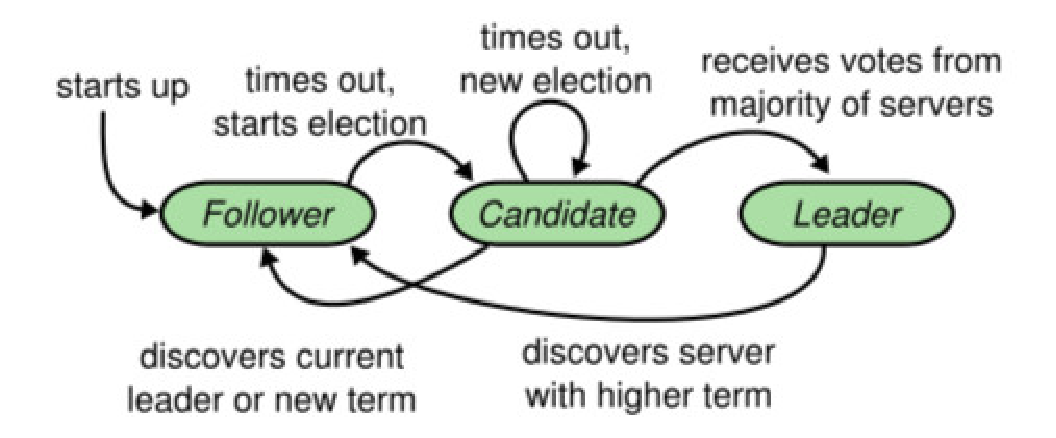
\includegraphics[width=.47\textwidth]{img/raft_server_states}}
    \caption{États et transitions dans un cluster Raft}
    \label{fig:raft_server_states}
%\end{wrapfigure}
\end{figure}

Les \emph{followers} ne font que répondre aux requêtes des autres serveurs. Si
un \emph{follower} ne reçoit plus de communications, il devient alors
\emph{candidat} et initie une élection. Le \emph{candidat} qui reçoit les votes
d'un majorité du cluster complet devient le nouveau \emph{leader}. D'une manière
générale, les \emph{leaders} opèrent jusqu'à ce qu'ils échouent.

\section{Élection d'un \emph{leader}}

Comme le montre la figure \ref{fig:leader_election}, le temps est divisé en
termes. Chaque terme commence par une élection. Après une élection fructueuse,
un \emph{leader} unique gère l'intégralité du cluster jusqu'à la fin du terme.
Parfois les élections échouent, auquel cas le terme se terminera sans choisir de
\emph{leader} et de nouvelles élections auront lieu au prochain terme. Il est
important de noter que les transitions seront observées à des moments différents
d'un serveur à l'autre.

%\begin{wrapfigure}{r}{.4\textwidth}
\begin{figure}[H]
    \centerline{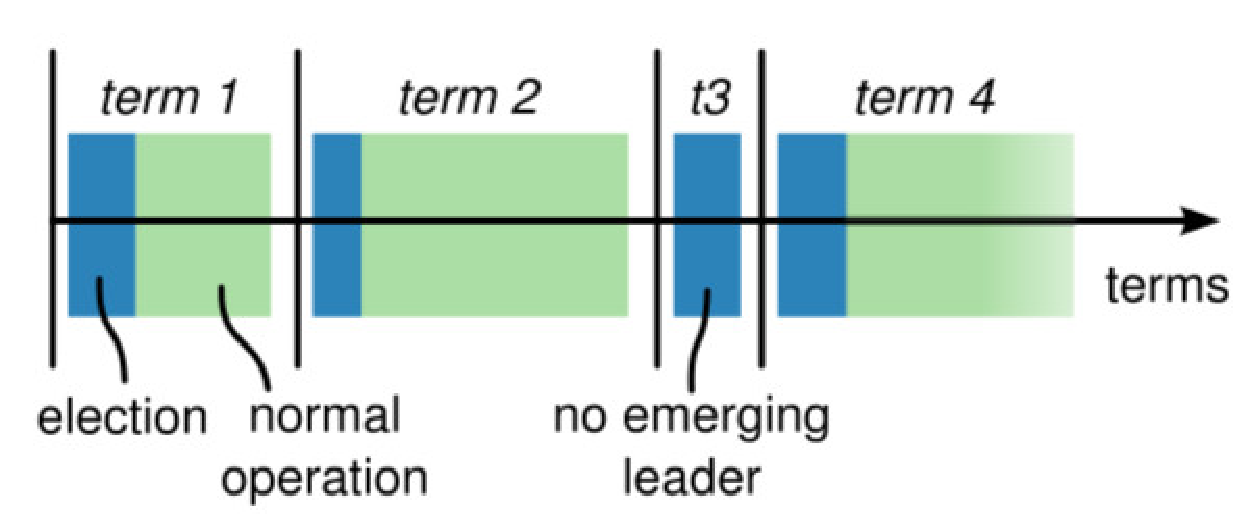
\includegraphics[width=.37\textwidth]{img/leader_election}}
    \caption{Processus d'élection d'un \emph{leader}}
    \label{fig:leader_election}
%\end{wrapfigure}
\end{figure}

\section{Réplication des journaux}

L'organisation des journaux est détaillée par la figure
\ref{fig:log_replication}.  Les journaux sont composés d'entrées
séquentiellement numérotées. Dans notre gestionnaire de contexte, ces entrées
correspondent à des états incrémentaux de notre ontologie. Chaque entrée réfère aux terme
durant lequel elle a été créée (le numéro de case dans la figure
\ref{fig:log_replication}) et contient une commande pour la machine à état. Une
entrée est considérée comme \emph{une transaction validée (committed)} si son
insertion dans la machine à état est sans dangers.

%\begin{wrapfigure}{r}{.4\textwidth}
\begin{figure}[H]
    \centerline{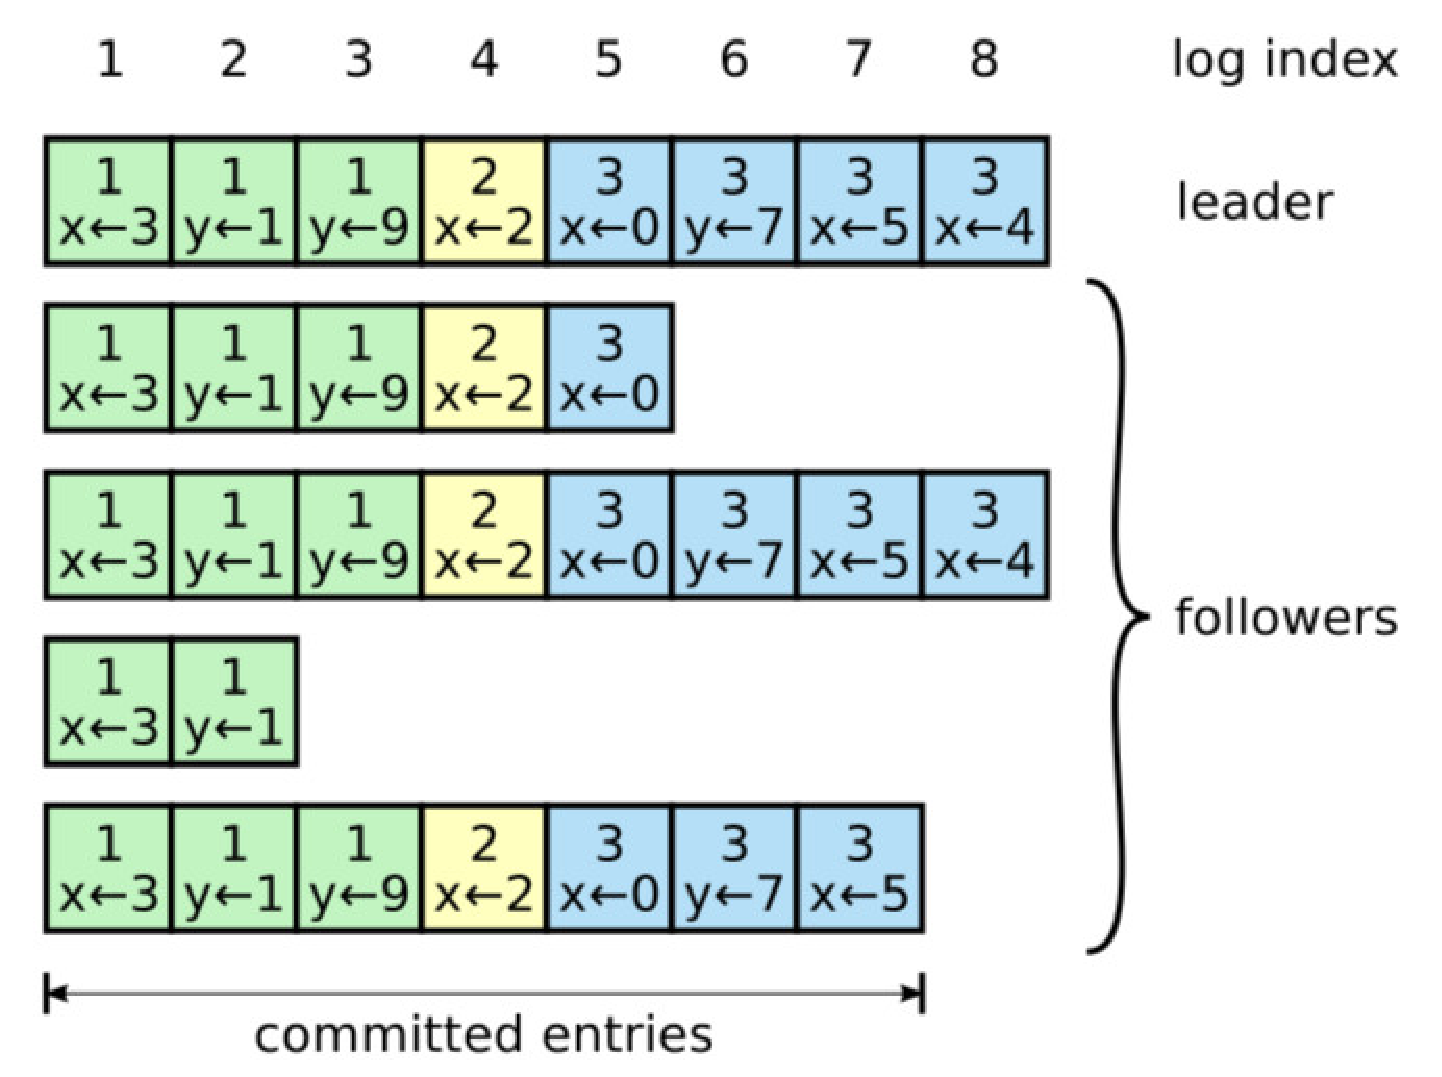
\includegraphics[width=.37\textwidth]{img/log_replication}}
    \caption{Processus de réplication des journaux}
    \label{fig:log_replication}
%\end{wrapfigure}
\end{figure}

En cycle fonctionnement normal, il y a un et un seul \emph{leader} et $n$
\emph{followers}. Le \emph{leader} envoie des pulsations régulières, témoins de
sa disponibilité, aux autres membres du cluster. Le premier \emph{follower}
remarquant l'inactivité du \emph{leader} (arrêt des pulsations) initie alors de
nouvelles élections. 

%%%%%%%%%%%%%%%%%%%%%%%%%%%%%%%%%%%%%%%%%%%%%%%%%%%%%%%%%%%%%%%%%%%%%%%

\chapter{Interface d'administration}
\label{appendix:interface}

\section{Interface pour les définition des variables de configuration de bas
niveau}
\label{appendix:interface_genconfig}

\begin{figure}[H]
    \centerline{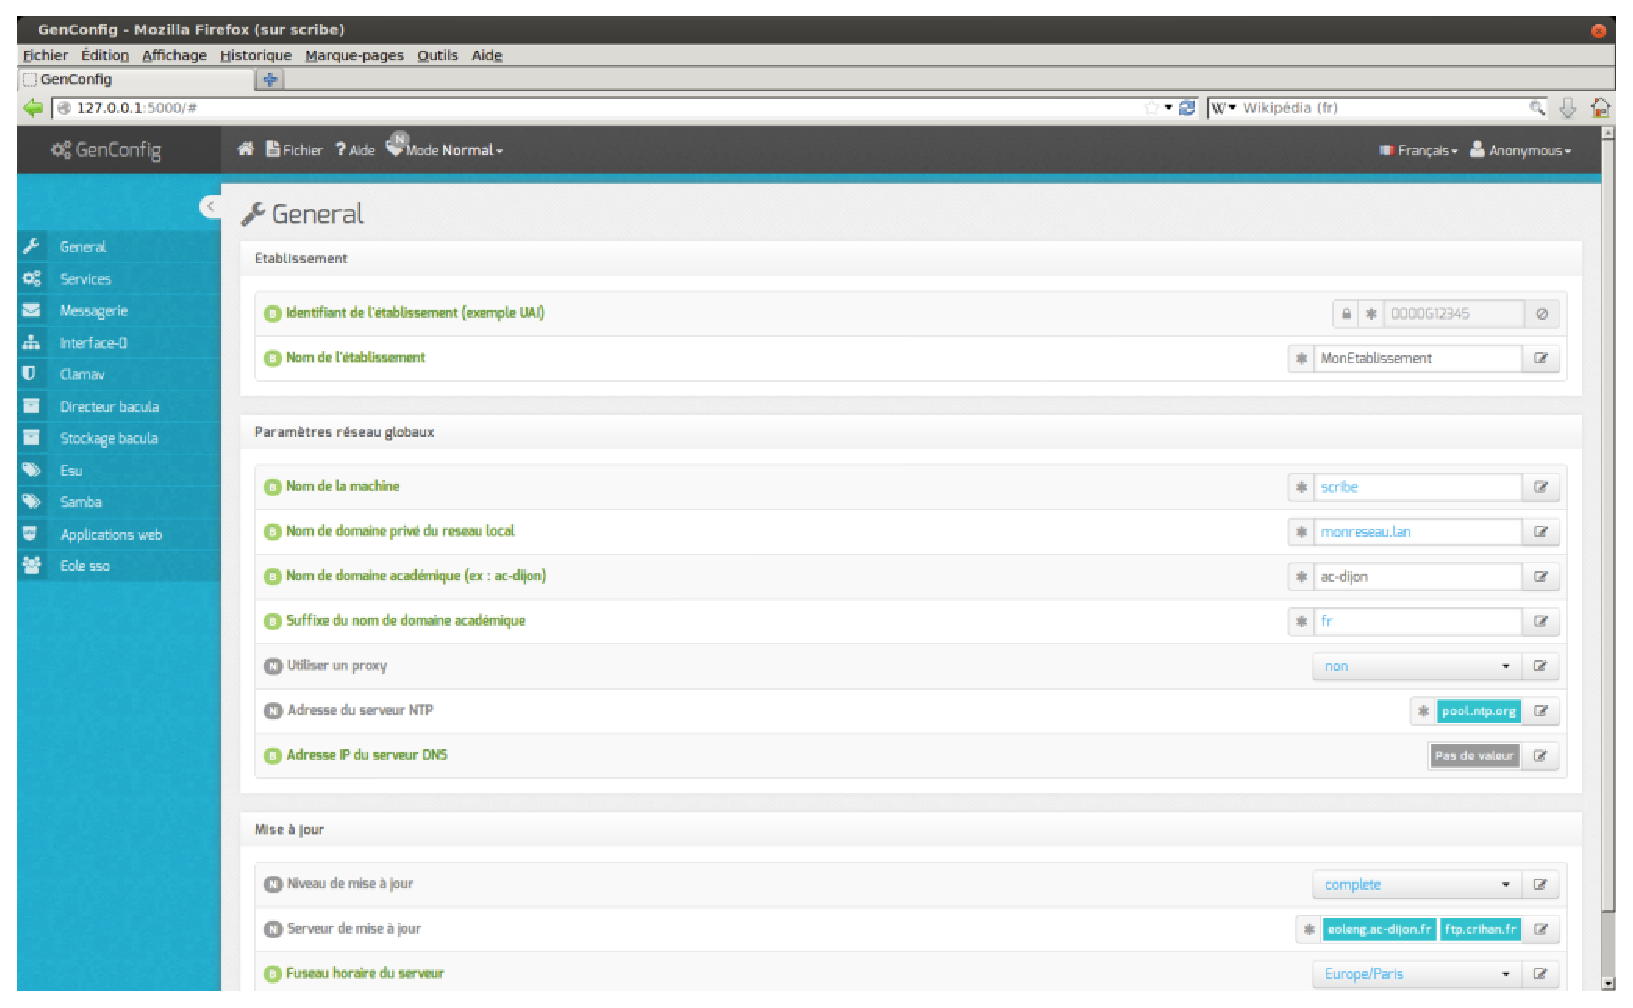
\includegraphics[width=\textwidth]{img/gen_config}}
    \caption{Interface d'administration du gestionnaire de configuration}
    \label{fig:gen_config}
\end{figure}

\section{Interface pour la consultation de l'ontologie}
\label{appendix:interface_query}

\begin{figure}[H]
    \centerline{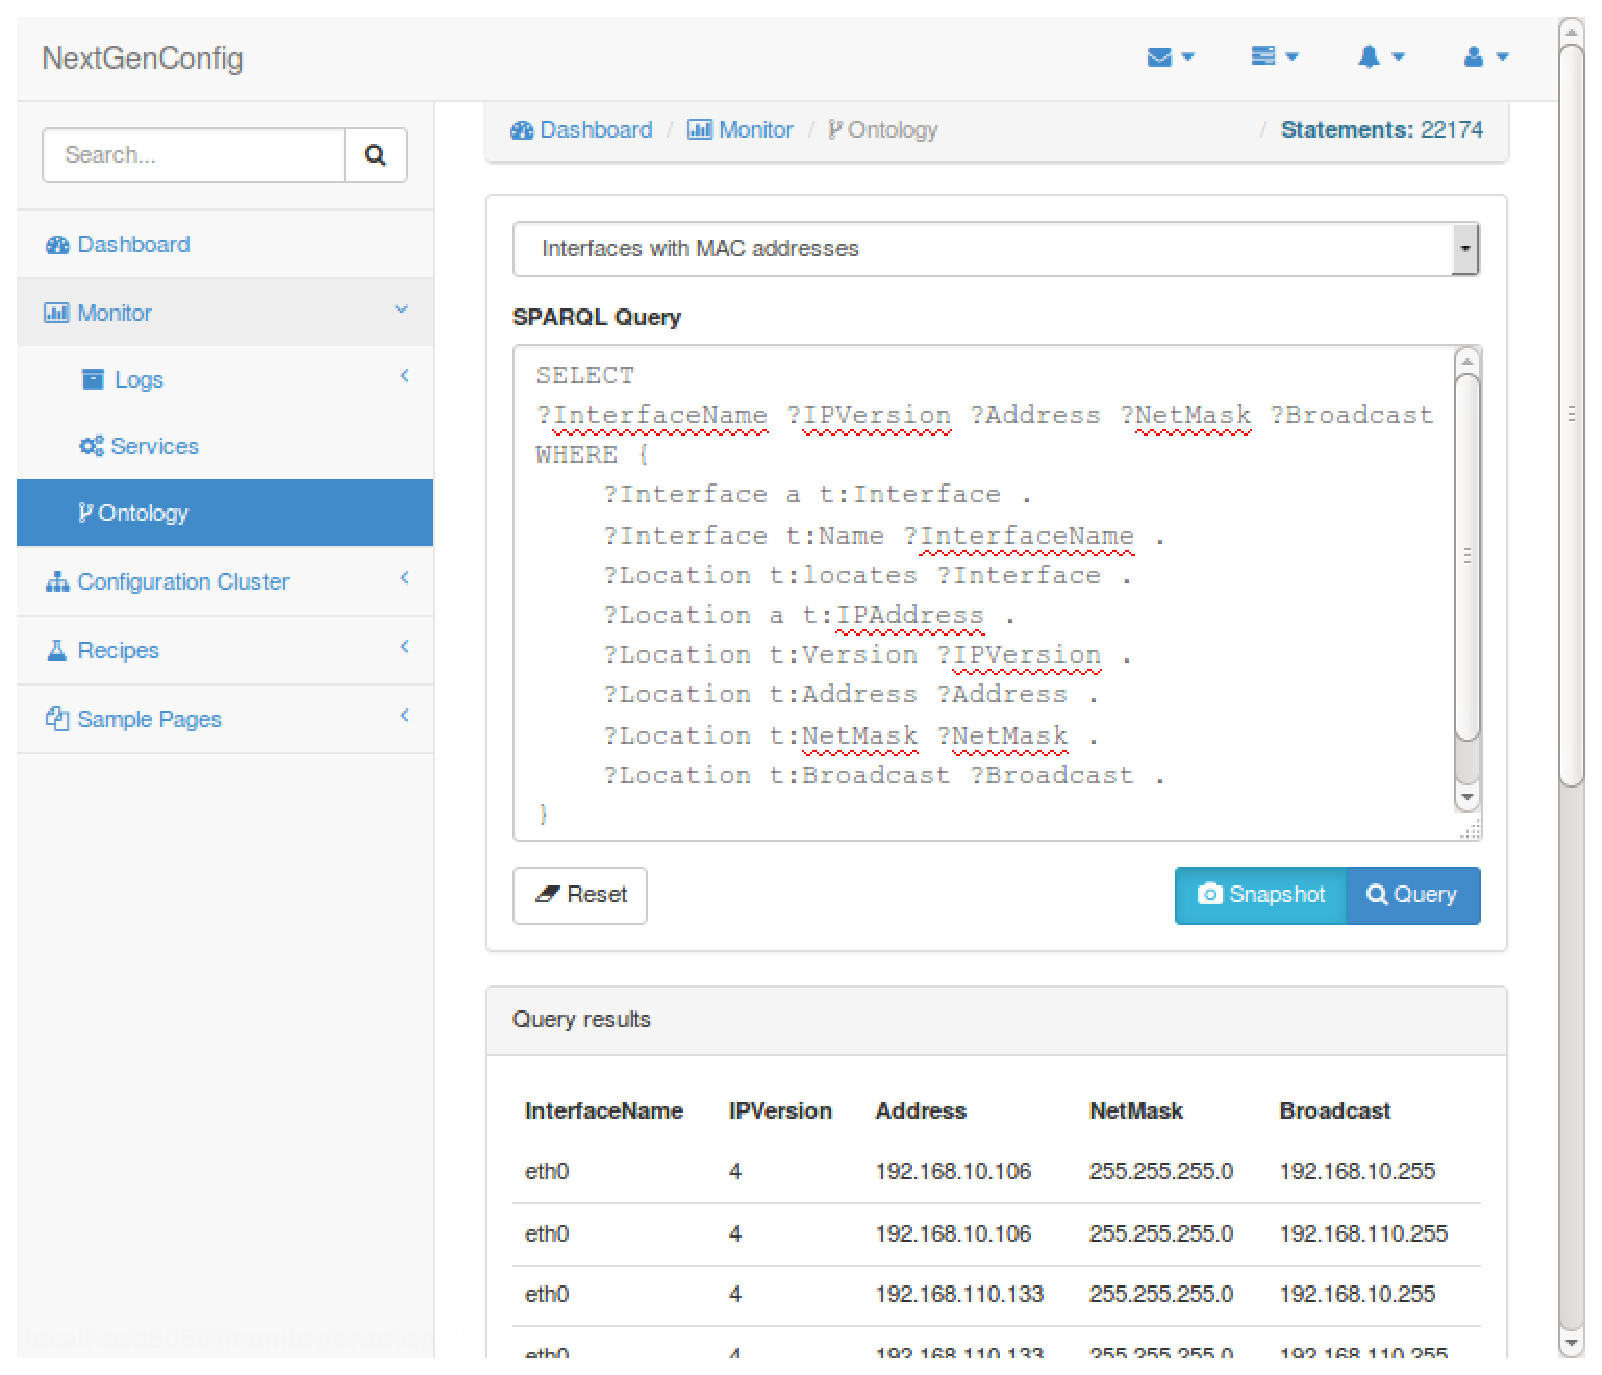
\includegraphics[width=\textwidth]{img/trifle_gui}}
    \caption{Interface d'administration du gestionnaire de configuration}
    \label{fig:trifle_gui}
\end{figure}


%%%%%%%%%%%%%%%%%%%%%%%%%%%%%%%%%%%%%%%%%%%%%%%%%%%%%%%%%%%%%%%%%%%%%%%

\chapter{Présentation d'EOLE}
\label{appendix:EOLE}

\section{Introduction}

Eole est un projet collaboratif basé sur la philosophie du logiciel libre.

La mutualisation des compétences et des moyens permet de réaliser des solutions
économiques, fiables et performantes.

\paragraph{EOLE} propose des solutions clef en main pour la mise en place de
serveurs Intranet/Internet.

Ces réalisations s’insèrent dans le cadre de réflexions et de recommandations
d’un certain nombre de structures et d’organismes ministériels favorables à
l’usage des logiciels libres dans l’administration.

\section{Modules EOLE}\label{modules eole}

Chaque module constitue une distribution GNU/LINUX spécifique qui permet
d’installer facilement un serveur dédié. Les services offerts sont
pré-configurés, l’ensemble est cohérent. Vous devez télécharger sur ce site
l’image ISO qui vous permettra de graver un DVD ou un CD d’installation. Ce
DVD/CD est multi module, le choix du module à installer est proposé au
démarrage (boot). 

\subsection{Amon}

Protéger les utilisateurs et les équipements.

Le pare feu Amon permet de partager en toute sécurité un accès Internet 
entre les sous réseaux d'un réseau local.

Installé sur un serveur dédié, équipé de deux, trois, quatre ou cinq 
interfaces réseau, il permet d'organiser au mieux votre réseau.
Des modèles de règles de pare feu sont disponibles pour chaque architecture.
Vous pouvez les utiliser tels quels ou bien les modifier à votre convenance. 
Un outil spécifique, Era, est à disposition pour effectuer ce travail.

\subsubsection{Principales fonctionnalités d'Amon}

\begin{itemize}
  \item Routage
  \item Support Vlan
  \item Authentification des utilisateurs
  \item Filtrage réseau
    \begin{itemize}
      \item Par IP (netfilter)
      \item par utilisateur (NuFW)
    \end{itemize}
  \item Filtrage de site amélioré
    \begin{itemize}
      \item Listes de sites interdits mises à jour quotidiennement
      \item Analyse sémantique des pages consultées
    \end{itemize}
  \item Réseau virtuel privé
  \item Suivi détaillé de la navigation web
  \item Mises à jour automatiques
  \item Journalisation des fichiers logs
  \item Détection d'intrusions
  \item Service de cache web
  \item Administration simplifiée
  \item Statistiques sur l'état du système
  \item Statistiques d'utilisation
\end{itemize}   

\subsection{Scribe}

Scribe est un contrôleur de domaine dotée de fonctions évoluées. 
Il optimise la gestion de votre parc de stations clientes.

Il dispose d'un annuaire qui référence, élèves, parents, personnels 
enseignant et administratifs, il propose un service de messagerie et héberge 
vos applications web au sein d'un portail Web 2.0

\subsubsection{Scribe est un contrôleur de domaine}

\begin{itemize}
  \item Gestion des connexions réseau des utilisateurs
  \item Partage de fichiers et de répertoires
  \item Support des ACL
  \item Partage d'imprimantes
  \item Gestion des comptes utilisateurs et des accès
  \item Gestion quotas disques et d'impression
  \item Exécution d'applications utilisateurs
\end{itemize}

\subsubsection{Scribe est un système de messagerie articulé autour d'un 
               annuaire performant}

\begin{itemize}
  \item L'annuaire est initialisé à partir d'importation de comptes 
        (SCONET, BE1D, AAF, CSV,...)
  \item L'annuaire peut servir de base d'authentification pour d'autres 
        services réseaux
  \item La messagerie gère deux domaines distincts (l'Internet et 
        l'intranet académique)
  \item Utilisation au choix d'une interface web multilingue ou d'un 
        client de messagerie standards
  \item Un service de listes de diffusion
  \item Une sécurité anti spam, un anti virus, une gestion de quotas 
        (taille des boites aux lettres)
\end{itemize}

\subsubsection{Scribe offre des services web => Envole 2.0}

\begin{itemize}
  \item Un serveur web
  \item Un portail web
  \item Des applications pré-installées
\end{itemize}

\subsubsection{Scribe est un serveur d'authentification unqiue (SSO)}

\begin{itemize}
  \item Eole SSO utilise l'annuaire LDAP
  \item Les standards C.A.S 2 et OpenID son supportés
  \item La fédération d'identité est possible via le protocole SAML
\end{itemize}

\subsubsection{Scribe dispose d'une gestion avancée des utilisateurs et 
               des postes clients}

\begin{itemize}
  \item Distribution de devoir
  \item Contrôle d'accès à Internet et au services réseaux
  \item Appliquer des restrictions ou pré configurer des applications, en
        fonction du login de l'utilisateur ou de ses groupes et du nom de 
        la machine sur laquelle il se connecte
  \item Effectuer des actions distantes sur les stations (fermer la 
        session, éteindre ou redémarrer un ou plusieurs postes)
  \item Surveiller la détection de virus par le serveur
\end{itemize}


\subsection{Horus}

Le module Horus est un contrôleur de domaine pour le réseau administratif 
d'un établissement scolaire ou d'un service académique.

Il offre toutes les fonctionnalités de partage de fichiers et d'imprimantes.

Il est également utilisable dans n'importe quelle autre structure 
nécessitant un contrôleur de domaine.

Un contrôleur de domaine est un serveur central qui est en charge des 
contrôles d'accès.

Un domaine est une entité logique qui reflète le plus souvent une 
organisation hiérarchique. Le domaine permet à l'administrateur système de 
gérer efficacement les utilisateurs des stations déployées car les 
informations (comptes et autorisations d'accès) sont centralisées dans une 
même base de données.

Le contrôleur de domaine permet donc :

\begin{itemize}
  \item De gérer des comptes utilisateur : ajouter, supprimer et modifier 
        un utilisateur
  \item De créer des groupes d'utilisateurs : créer des groupes pour 
        simplifier la gestion des politiques (permission sur des dossiers, 
        permission sur des services,...)
  \item De créer des politiques de sécurité qui seront appliquées aux 
        utilisateurs et aux groupes d'utilisateurs.
\end{itemize}            
 
L'utilisateur peut, sur une machine cliente raccordée au réseau, faire le 
choix de démarrer une session avec un compte du domaine ou avec un compte 
local s'il en existe. Il est ainsi possible d'ouvrir une session sur 
n'importe quel poste du domaine.

\subsection{Éclair}

Eclair est un serveur de clients légers linux.

Il permet de faire démarrer, depuis le réseau, des machines sans système
d'exploitation installé.

En pratique le serveur est la seule machine ayant un système installé, c'est 
lui qui exporte son système vers les clients légers. Tout ceci est 
complètement transparent pour l'utilisateur, il utilise le client léger, on 
dit aussi terminal, exactement comme s'il utilisait un ordinateur normal.

Tout le système et toutes les applications disponibles sur les terminaux étant
en fait installés sur le serveur, il n'y a qu'une seule machine à administrer.
Si vous installez une application sur le serveur, elle sera
immédiatement disponible pour tous les clients légers.

\subsection{Amon École}

Un seul serveur pour plusieurs modules.

Cela permet aux établissement d'avoir différents services sur une même machine
physique au lieu de multiplier le nombre de serveurs.

De ce fait, AmonEcole est particulière adapté aux petites structures en
termes d'effectif ou de moyens comme les écoles primaires ou les petits
collèges.

Il est également possible d'installer les module Horus (serveur de fichier)
et Eclair (clients légers)

En version 2.2 ces différents modules sont installés sur une seule machine
physique grâce à la technique de virtualisation (OpenVZ).

En version 2.3 on utilise le mode conteneur (LXC)

\subsection{Sphynx}

Le serveur Sphynx est un concentrateur de réseau virtuel privé.

Intégrant des composants logiciels de haute disponibilité, Sphynx vous permet
de relier en réseau vos serveurs pour former un réseau virtuel privé (RVP) 
avec le pare feu Amon dans les établissements distants et Sphynx en entrée de 
votre réseau.

Il fait parti des éléments constitutifs du réseau AGRIATES (Intranet Sécurisé
entre les Académie et les Etabissements scolaires).

\subsection{Zéphir}

Le module Zéphir propose une solution normalisée pour faciliter le
déploiement, la surveillance et la maintenance des modules EOLE.

Zéphir héberge une base de données des établissements et des serveurs 
installés dans ces établissements.

Zéphir permet la gestion de la configuration des serveurs

\begin{itemize}
  \item La génération des configurations serveurs (création du dictionnaire)
  \item Le stockage de ces configurations (fichier.eol)
  \item La distribution des ces configurations sur les serveurs via le réseau
  \item La mise à jour des configurations avec une gestion des différentes 
        versions et un historique des modifications effectuées
  \item Le lancement d'actions à distance
\end{itemize}

Zéphir dispose d'un module de surveillance de vos serveurs dans les 
établissements. Il permet la remontée d'alertes à intervalles réguliers. 
Des actions sur les serveurs en alerte peuvent être lancées automatiquement 
si besoin.


% ex: set spelllang=fr spell: %
%%% Local Variables: ***
%%% mode: latex ***
%%% TeX-master: "thesis.tex" ***
%%% End: ***
